\documentclass[12pt]{article}
\usepackage[a4paper,margin=.5in]{geometry}
\usepackage{graphicx}
\usepackage{booktabs}
\usepackage{listings}
\usepackage{color}

\definecolor{dkgreen}{rgb}{0,0.6,0}
\definecolor{gray}{rgb}{0.5,0.5,0.5}
\definecolor{mauve}{rgb}{0.58,0,0.82}

\lstset{frame=tb,
  language=Python,
  aboveskip=3mm,
  belowskip=3mm,
  showstringspaces=false,
  columns=flexible,
  basicstyle={\small\ttfamily},
  numbers=none,
  numberstyle=\tiny\color{gray},
  keywordstyle=\color{blue},
  commentstyle=\color{dkgreen},
  stringstyle=\color{mauve},
  breaklines=true,
  breakatwhitespace=true,
  tabsize=3
}
%\usepackage{subfig}
\usepackage{subcaption}
\usepackage{hyperref}
\hypersetup{
    colorlinks=true,
    linkcolor=blue,
    filecolor=magenta,      
    urlcolor=cyan,
    pdftitle={Overleaf Example},
    pdfpagemode=FullScreen,
    }
\newcommand*{\figuretitle}[1]{%
    {\centering%   <--------  will only affect the title because of the grouping (by the
    \textbf{#1}%              braces before \centering and behind \medskip). If you remove
    \par\medskip}%            these braces the whole body of a {figure} env will be centered.
}
\title{Exam 1}

\author{Tylman Michael\\CSE 546 Machine Learning}
\date{2/24/2023}
%moderncv theme
\usepackage[utf8]{inputenc} 
\begin{document}
\maketitle{}
\section{Problem 1}
\begin{figure}
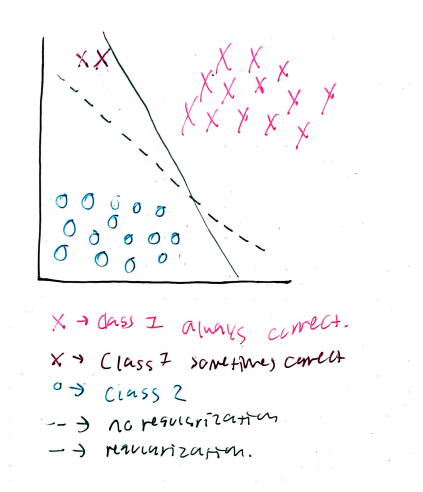
\includegraphics[width=.65\textwidth]{../results/Prob_1_plot.PNG}
\caption{Plot for Problem 1}
\label{image1}
\end{figure}
The image for this plot is in Figure  \ref{image1}. The reason why these samples can be correctly classified without any 
regularization is because the SVM will look to maximize the margin which results in 0 items missed without any care for
the fact that these 2 points are outliers. However, once we start to use regularization, it lowers the impact of outliers
on our decision boundary, which \emph{could} result in the decision boundary moving to favor a cleaner margin between 
the two easier clusters.
\subsection{a)}
Solution b can be better than solution a if those two points really are outliers. If they are a poor indication of the 
general behavior of the phenemenon being studied, then they should not be allowed to have such a strong impact on the 
learned decision boundary of our model. We want regularization to make our model less sensitive to outliers.

\subsection{b)}
Solution a can be better than solution b if those two points are not outliers, but rather our training set overall is 
a poor indicator of the behavior of the phenomenon. If class A actually was bimodal in behavior, with 2 possible clusters 
with a probability of 13/15 for the larger, and 2/15 for the smaller, then our data is a perfect model of the phenomenon 
and every point should be considered. Interstingly enough, an example of something bimodally distributed is DNA Methylation,
which I worked on previously before coming to UofL. This can be seen in figure 2 of the paper located 
\href{https://bmcbioinformatics.biomedcentral.com/articles/10.1186/1471-2105-11-587}{Here}
if you're interested in learning more. 


\section{Problem 2}
\begin{figure}
  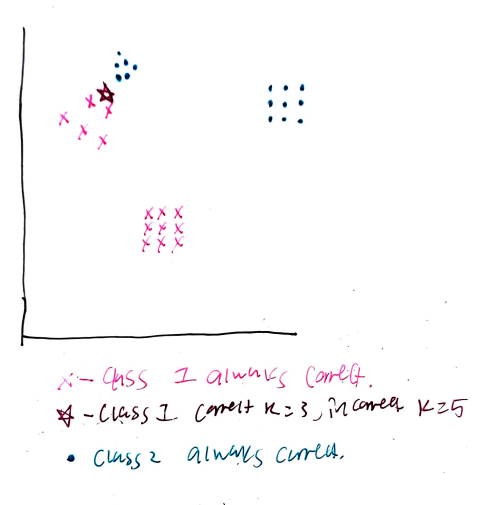
\includegraphics[width=.65\textwidth]{../results/Prob_2_plot.PNG}
  \caption{Plot for Problem 2}
  \label{image2}
\end{figure}

The sample which cannot be classified correctly is shown in Figure \ref{image2} as the darker pink star. I drew this
such that 2 of the 3 nearest neighbors are of the correct class, such that it will work with k=3, but then 3 of the nearest
5 neighbors are of the wrong class such that it will not classify correctly with k=5. I then padded the 2 correct and the 
3 incorrect neighbors with enough of the same class such that they would have enough neighbors close by that they will 
entirely fill the all of the top 5 closest neighbors with members of the same class to ensure they would be classified as 
correct. 

Then, to not muddy the water with my work, I placed the remaining 9 members of each class in a little grid off on their own 
such that they would be trivial to see that they are going to be correctly labelled.

\section{Problem 3}
\subsection{a)}
I would employ the Naive Bayes classifier for this data primarily due to the following two reasons.

1. The amount of blue dots that are floating above the 
orange cluster, along with the small shared barrier of orange and blue markers to the left of the orange cluster, would 
be regions where a KNN classifier would likely struggle, and no clear linear boundary exists that can outperform a classifier
that considers the floating points above the orange cluster. 

2. The data seems to vaguely be normally distributed around 2 means, with the orange dataset having an extremely small 
variance compared to that of the blue data.


Since this dataset seems to meet the assumptions taken by a Naive Bayes classifier, and has evidence of areas where other 
models would likely struggle, I think the Naive Bayes classifier would perform very well on this dataset. It may be possible 
that a decision tree-based approach (with a random forest or gradient boosted model) could perform as well as a Naive Bayes
classifier, but these trees can be longer to train and require more memory if we were to grow this dataset. 

I don't think 
that the supposed performance gained (if any!) would be enough to overcome how well the Naive Bayes classifier fits this 
application, and I suspect they would have poorer generalization. For example, if we were to have unknown samples below the
orange cluster, to the right of the little outcropping of blue dots, I think they would more likely belong to the blue class.
In this case, the Naive Bayes classifier would accurately assess these new samples, but the decision trees would likely not.


\subsection{b)}
I'd definitely choose a decision-tree based approach for this dataset. The KNN models would struggle on the sparse blue 
dots that are on the edges around the more tightly-packed orange dot. The blue dots don't have any strongly defined 
mathematical distribution that makes it seem like we could leverage a Naive Bayes classifier, nor do the orange dots appear
to be normally distributed. There is no one line of separation, unless we were to use a nonlinear projection about the centroid
of the orange class, probably with a radial basis function (which we haven't covered).

With all of that in mind, the orange class can be cleanly separated into a box which surrounds it on all sides that 
also does not include any blue dots. This leads me to believe that a decision-tree based approach would likely work very well.
I'd have to say to go with a standard random forest approach over a gradient boosted approach purely because this seems to 
be a rather simple dataset that we could get great performance on with a random forest with faster training time than 
with a gradient-boosted classifier. 

\section{Problem 4}
For every model in problems 4 and 5, I chose to use a combination of a scaler and a normalizer to force all of the data 
onto a unit sphere around the origin. This might have been a poor choice for some models, but due to time constraints 
I decided it would be better to do the data normalization that I was the most comfortable with understanding conceptually
since the focus of this exam is on the models themselves, and not the preprocessing.


I will list a single table with the best results (with the param lists cut) for every model for ease of reference 
in Table \ref{table1}. The most important rows to recognize are the last few, where best\_final\_test is the accuracy 
of the best\ model on the test set, best\_cv\_test and best\_cv\_train are the average test accuracies of the best model
 across the CV splits for test and train respectively. A couple of those values are available earlier in the table as well,
 but I included them at the all together for ease of use. 

Additionally, I did do a 4-fold cross-validation for all questions in problem 4 simply because my code assumed that it 
would be working on cross-validation folds, and it was easier to just make my machine work 4x as hard instead of fixing my 
code to allow for no cross-validation.

\begin{table}
  \resizebox*{.95\textwidth}{!}{\begin{tabular}{lllllll}
\toprule
{} &                   stack &                  NBbag &                 mlpbag &                  NBada &                treeada &                  SVMbag \\
\midrule
Index                       &                       2 &                    867 &                     14 &                     51 &                     47 &                      17 \\
mean\_fit\_time               &      1405.5506918430328 &     40.285290360450745 &      579.3783206343651 &     102.77094876766205 &      1229.745915234089 &      129.07705068588257 \\
std\_fit\_time                &       56.74206058134601 &     0.6317175670817758 &      7.455601391413241 &     0.8867015999451987 &     1.8724155730382983 &       9.796660667519168 \\
mean\_score\_time             &      11.178422927856445 &      51.00288212299347 &     0.5981229543685913 &     48.676812052726746 &      3.830958664417267 &      27.196506679058075 \\
std\_score\_time              &       1.405742496910865 &     1.8923625091969507 &    0.11387845129075089 &     1.8198226356237728 &    0.28462153313195493 &       4.294021210732005 \\
mean\_test\_accuracy          &                    0.79 &     0.5754999999999999 &                0.79525 &                  0.637 &                0.54825 &                 0.77575 \\
std\_test\_accuracy           &   0.0022360679774997916 &   0.019868316486305507 &   0.008525696452489974 &    0.01383835250309806 &     0.0067961386095341 &     0.00831790237980707 \\
rank\_test\_accuracy          &                       5 &                     44 &                      1 &                      1 &                      1 &                       2 \\
mean\_train\_accuracy         &      0.9977499999999999 &                0.62925 &     0.9940833333333333 &     0.8125833333333333 &                  0.764 &                 0.99425 \\
std\_train\_accuracy          &   0.0007592027982620297 &   0.004872684635347887 &  0.0009537935951883014 &    0.01061281981588514 &    0.01018713785995741 &   0.0008620067027324092 \\
mean\_test\_f1\_weighted       &      0.7912570496724283 &     0.5858494831502836 &     0.7949238630429338 &     0.6431246854754509 &     0.5576218846400178 &      0.7762111731817483 \\
std\_test\_f1\_weighted        &   0.0029872474406088608 &    0.01903181076309097 &   0.008385994462715676 &   0.012909250517893546 &   0.007753848653095678 &    0.009018811244895598 \\
rank\_test\_f1\_weighted       &                       3 &                     38 &                      1 &                      1 &                      1 &                       2 \\
mean\_train\_f1\_weighted      &      0.9977507823245164 &     0.6389193533117794 &     0.9940841593977978 &     0.8137017737836371 &     0.7653651061845691 &      0.9942576816522287 \\
std\_train\_f1\_weighted       &   0.0007583764213535456 &   0.005289021391854054 &  0.0009541156349656866 &   0.010307792046297188 &   0.010124753277141824 &   0.0008584699193975221 \\
mean\_test\_roc\_auc\_ovr       &      0.9730999015536933 &     0.9088672548387857 &     0.9749867328830162 &     0.9364586653065938 &     0.8743949551758458 &      0.9688421608215558 \\
std\_test\_roc\_auc\_ovr        &    0.000915550433627727 &   0.006604637647041263 &  0.0008938521311151068 &  0.0030788513632281837 &  0.0034540071161737835 &   0.0019750940256677376 \\
rank\_test\_roc\_auc\_ovr       &                       1 &                      1 &                      1 &                      1 &                      1 &                       1 \\
mean\_train\_roc\_auc\_ovr      &      0.9999612015765678 &     0.9389531956927522 &     0.9999600333256833 &     0.9844012423207428 &      0.949929571828595 &       0.999923288362849 \\
std\_train\_roc\_auc\_ovr       &  2.4671281578632394e-05 &  0.0030594180625836366 &  1.558742578374733e-05 &  0.0010215200718514444 &   0.002438923495362692 &  3.1182187144615235e-05 \\
best\_final\_test\_accuracy    &                    0.96 &                  0.602 &                  0.961 &                   0.75 &                  0.714 &                   0.791 \\
best\_final\_test\_roc\_ovr     &      0.9989464604987599 &      0.927274695189538 &      0.996860066599987 &     0.9706142287135784 &     0.9326248076880352 &      0.9701864899787338 \\
best\_final\_test\_f1\_weighted &      0.9600616632865854 &     0.6136405868499072 &     0.9609942113384318 &      0.752537870834654 &     0.7160316970317154 &      0.7909626666332018 \\
\bottomrule
\end{tabular}
}
  \caption{Best Results and MetaData}
  \label{table1}
\end{table}

\subsection{Ridge Regression}
For the Ridge Regression classifier, I did not have a discrete that I could use to group my data and label it with 
my pre-existing software. So, I kluged a patch in order to make my plotting structure work without a grouping variable.
I will certainly find a better solution for it in the future, but due to the time constraints we will have to work with 
it for now.

The results of my cross validation for the Ridge Regressor are shown in Figure \ref{figure1}. I have included the time
complexity required as well as the mean performance. As we can see, the alpha parameter initially gave some boost to 
accuracy, but then caused a steady drop in accuracy as it increased. However, the effect of this is overly illustrated
on the plot by the automatic choice of y-boundaries. If we look closely, we can see that alpha actually did not  have 
much of an appreciable effect on the performance of the model. 

The top and bottom of our graph are a mere .35 percent apart from one another. Admittedly, we can see the difference 
between the training and the test curve decrease as we alpha increases, so it is lowering overfitting. But, it's really 
not accomplishing much. 

We can see that the best result for our ridge regressor occurs when alpha is .021, but as we stated earlier it does not 
make much of a difference. However, we can say that there is little to no overfitting occuring, considering the fact 
that the mean test score and mean train score are within each other's standard deviation. This woudl be a great plus in favor 
of the ridge regressor, if it had performed better.

\begin{figure}
  \begin{subfigure}{.5\textwidth}
    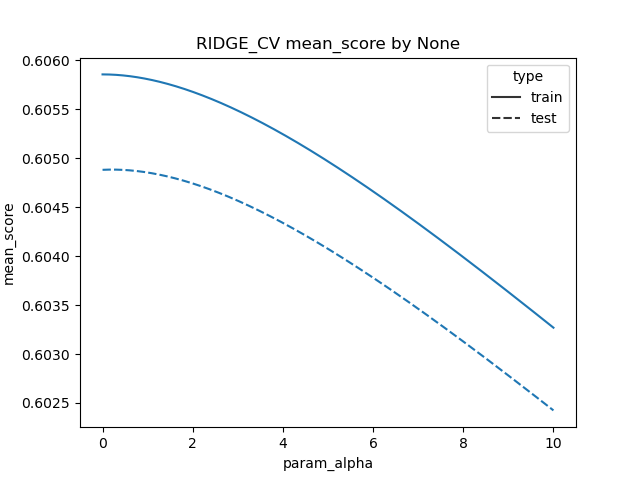
\includegraphics[width=.95\textwidth]{../results/Ridge_cv/None_mean_score_param_alpha.png}
    \caption{Ridge Regression Mean score}
    \end{subfigure}%
  \begin{subfigure}{.5\textwidth}
    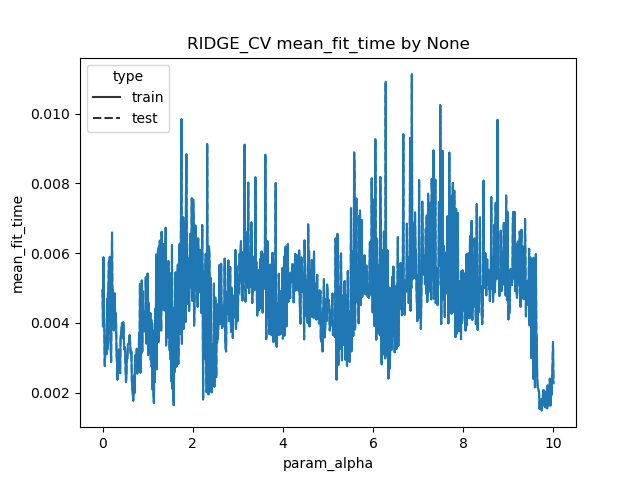
\includegraphics[width=.95\textwidth]{../results/Ridge_cv/None_mean_fit_time_param_alpha.png}
    \caption{Ridge Regression Average Train time.}
  \end{subfigure}
  \caption{Ridge Performance}
  \label{figure1}
\end{figure}

\subsection{Decision Tree}
The Decision Tree model (DT) suffered from a similar problem as the Ridge Regressor, so it also must deal with the kluged 
plotting problem. I also only varied the maximum depth pruning parameter, since the assignment only requested a parameter 
(not plural parameters), and there is no singular "pruning" parameter in sklearn. I have plotted the results of my training
in Figure \ref{figure2}

\begin{figure}
  \begin{subfigure}{.5\textwidth}
    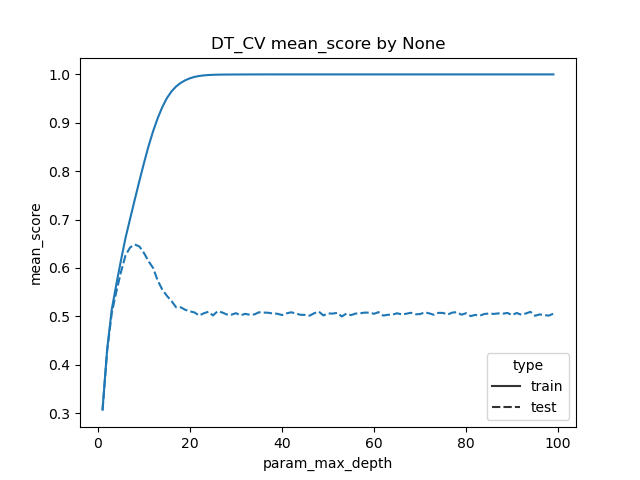
\includegraphics[width=.95\textwidth]{../results/DT_cv/None_mean_score_param_max_depth.png}
    \caption{DT Mean score}
    \end{subfigure}%
  \begin{subfigure}{.5\textwidth}
    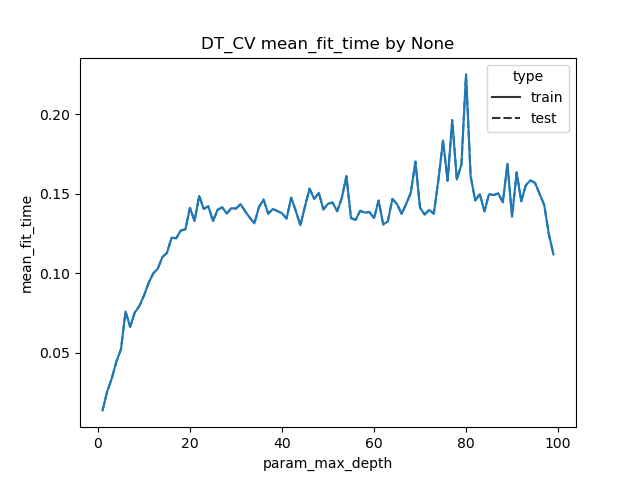
\includegraphics[width=.95\textwidth]{../results/DT_cv/None_mean_fit_time_param_max_depth.png}
    \caption{DT Average Train time.}
  \end{subfigure}
  \caption{DT Performance}
  \label{figure2}
\end{figure}

We can see here that the DT model saw great improvement up until a very clear maximum where the model began to classically 
overfit around a maximum depth of 8. At a max depth of 8, we got our best result as shown in Table \ref{table1}, which 
also showed only mild beginnings of overfitting. The overfitting continued to get worse from this point until about 
max depth of 20 where it seems like our model became fully overfit and saw no significant change for the rest of 
the experiment.

\subsection{Random Forest}
The Random Forest model (RF) did manage to have multiple items for me group by for my plotting software, so that's nice. 
As such, there will be four plots for the RF in Figure \ref{figure3}. Originally, I had my n\_estimators search go from 
100 to 700 in steps of 100, but I discoverd that the model was already very far overfit by the very first datapoint. 
Additionally, I had my max depth set to go from 10 to 100 in steps of 10, but the performance plateau'd already at 20.
So, I re-ran this experiment with estimators ranging from 1 to 20,  and max\_depth ranging from 1 to 30. This did increase
the total amount of time spent training, but I was able to work concurrently with the writeup and the training so that 
it wasn't too bad.

Once I did so, I found that the number of estimators capped out performance very quickly, reaching near peak performance 
at about 5 estimators, but slowly increasing until 20. I think if I had more time, I would have expanded my search past
25, but with my previous mistakes I had boxed myself into a corner.

Regardless, to explicitly stte the best parameters I had for the RF classifier, they are: "{'max\_depth': 18, 'max\_features': 'sqrt', 'n\_estimators': 20}"
Across every split, the log2 feature selection outperformed the sqrt feature selection. We can additionally see overfitting 
begin to occur before a maximum depth of 10, as the training and testing curves split from one another. 

Overall, the random forest performed well with moderate overfitting at the best selected model with a training accuracy 
of .947 and a testing accuracy of .75. However, it did generalize very well when applied to the test set, where it only 
lost .005 performance when going from the best average validation score to the test dataset.
\begin{figure}
  \begin{subfigure}{.5\textwidth}
    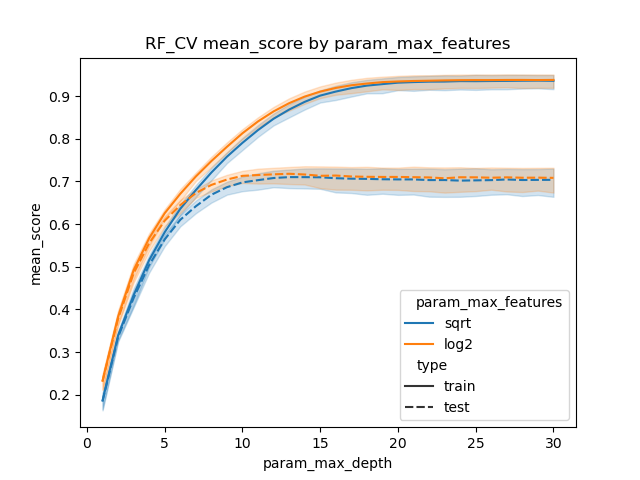
\includegraphics[width=.95\textwidth]{../results/rf_cv/param_max_features_mean_score_param_max_depth.png}
    \caption{RF Performance by Max Depth}
    \end{subfigure}%
  \begin{subfigure}{.5\textwidth}
    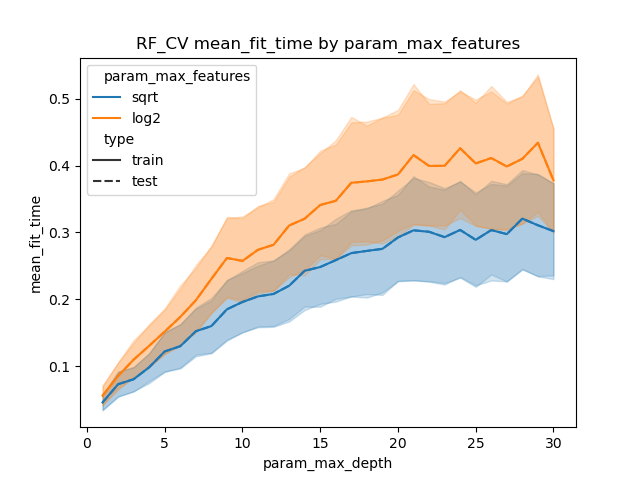
\includegraphics[width=.95\textwidth]{../results/rf_cv/param_max_features_mean_fit_time_param_max_depth.png}
    \caption{RF Average Fit Time by Max Depth}
  \end{subfigure}
  \begin{subfigure}{.5\textwidth}
    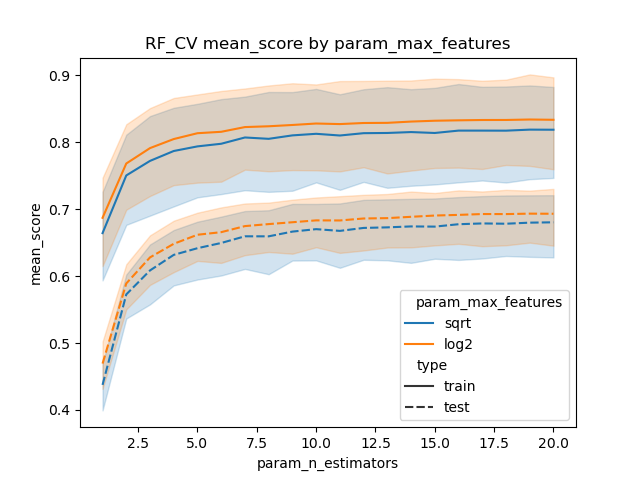
\includegraphics[width=.95\textwidth]{../results/rf_cv/param_max_features_mean_score_param_n_estimators.png}
    \caption{RF Performance by Estimators}
    \end{subfigure}%
  \begin{subfigure}{.5\textwidth}
    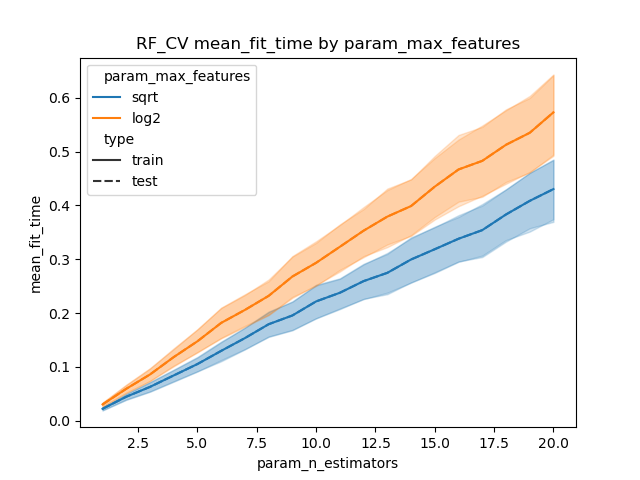
\includegraphics[width=.95\textwidth]{../results/rf_cv/param_max_features_mean_fit_time_param_n_estimators.png}
    \caption{RF Average Fit Time by Estimators}
  \end{subfigure}
  \caption{RF Performance}
  \label{figure3}
\end{figure}

\subsection{Comparison}
The random forest classifier comes out ahead, which is honestly to be expected when we consider our options. If our dataset
had any real complexity to it, a linear model likely might not be able to perform well. Additionally, it makes sense that 
a random forest of many decision trees will outperform a single decision tree for complex data. This also aligns with a comment
you made in class in regards to the random forest classifier being one of the best classifiers we will cover in this class with 
an extremely wide array of possible applications.

To make the feature importances more easily compared, I normalized the feature importances for each model. For the Ridge
regressor, I normalized the absolute value of the feature coefficient. The results of this can be seen in Figure 
\ref{figure4}. We can see that there's a consensus that Median Income is a strong driver of price, which makes a lot 
of sense. Essentially, rich people are very likely to spend more money on their homes. Something that surprised me was 
how much the Ridge regressor gravitated towards the average occupancy feature. I suppose that would be bounded into 
simpler discrete values likely in the range of 1 to 7 that can be simply measured with my normalization.

I think that the median income provides the most clear information that can be leveraged by a simple model, which is why
this feature so strongly dominates in the single decision tree model. However, I do see how the other features could provide
more complex information that a more advanced model can leverage which is why it doesn't dominate as much in the Random 
Forest model. Additionally, the Decision Tree is much more intentional about building it's one tree than the Random Forest 
is about building the multitude of trees it has. Therefore, the Random Forest model can afford to spend some energy on 
considering features that might not be as easily leveragable.

\begin{figure}
  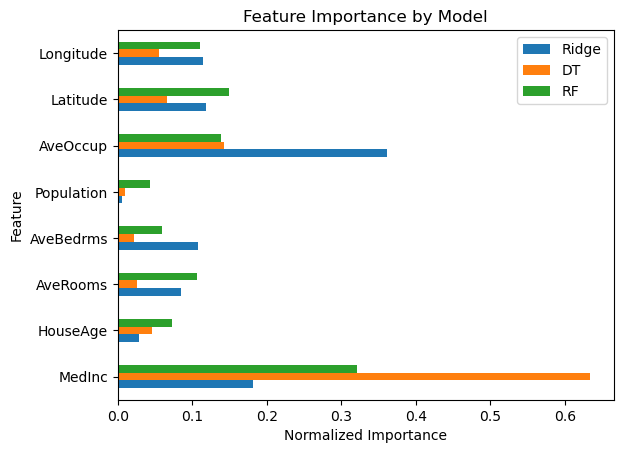
\includegraphics[width = .75\textwidth]{../results/Features.png}
  \label{figure4}
  \caption{Feature Importances}
\end{figure}


\section{Question 5}
\subsection{a)}
I used the same functionality as the previous questions to generate my results, which can be looked at in the accompanied
notebook. I will note, however, that my notebook will produce some additional plots if a model has multiple values that 
I mark as being and x value, which are accuracy contour plots. I've decided not to try and include these plots in my 
analysis, but you can feel free to look at them if you'd like to see exactly how two options interact with respect to 
their combined effect on accuracy.

\subsection{b)}
I am including my result for question 5 in it's own table in Table \ref{table2}, rather than lump it in with the others of question 
4. This is less space efficient, but better for readability.

Looking at the best result for the Gradient Boosted trees classifier (GB), we can see that this model is performing 
quite well. With a mean test score of .93 and mean train score of 1, this is a very promising result right out of the gate.
Looking at the behavior of parameters as shown in Figure \ref{figure5}, it appears that learning rate introduces a chaotic effect
when it is set too high, with the maximum depth providing some stabilization. 

Additionally, it appears that the higher maximum depth cleanly separates the performance across all factors, with the
order of performance nearly always being in the order of 5, 4, and then 3 with 5 being the best performance for the vast
majority of the parameters we attempted. However, it appears that the order actually inverts when we approach the optimal
performace point for each model. So, despite 4 and 5 beating 3 for most of the plot, the best performing model actually 
was a model with a maximum depth of 3. The optimal
parameters for this model are shown in Table 2 directly unlike the models in Table \ref{table1}. This is because I designed my table generation to include 
all options which are shared by all models. Since we are showing only 1 model in Table \ref{table2}, this means that all options are shown.

In terms of generalization, this model does very well. We are performing at a test accuracy of .916 with an average validation 
accuracy of .93. We did achieve a training accuracy of 1, which can be cause for concern regarding overfitting and generalization,
but it appears that these concerns are unwarranted given the validation and test accuracies.
I will admit, when I originally did this experiment with a much larger gridsearch, I found some models which 
performed moderately better. I chose to go with this analysis, since I was able to much better plot the performance with 
smoother continuity than when I had to skip the number of estimators in steps of 5 or 10.





\begin{table}
  \resizebox*{.4\textwidth}{!}{\begin{tabular}{lllllll}
\toprule
{} &                   stack &                  NBbag &                 mlpbag &                  NBada &                treeada &                  SVMbag \\
\midrule
Index                       &                       2 &                    867 &                     14 &                     51 &                     47 &                      17 \\
mean\_fit\_time               &      1405.5506918430328 &     40.285290360450745 &      579.3783206343651 &     102.77094876766205 &      1229.745915234089 &      129.07705068588257 \\
std\_fit\_time                &       56.74206058134601 &     0.6317175670817758 &      7.455601391413241 &     0.8867015999451987 &     1.8724155730382983 &       9.796660667519168 \\
mean\_score\_time             &      11.178422927856445 &      51.00288212299347 &     0.5981229543685913 &     48.676812052726746 &      3.830958664417267 &      27.196506679058075 \\
std\_score\_time              &       1.405742496910865 &     1.8923625091969507 &    0.11387845129075089 &     1.8198226356237728 &    0.28462153313195493 &       4.294021210732005 \\
mean\_test\_accuracy          &                    0.79 &     0.5754999999999999 &                0.79525 &                  0.637 &                0.54825 &                 0.77575 \\
std\_test\_accuracy           &   0.0022360679774997916 &   0.019868316486305507 &   0.008525696452489974 &    0.01383835250309806 &     0.0067961386095341 &     0.00831790237980707 \\
rank\_test\_accuracy          &                       5 &                     44 &                      1 &                      1 &                      1 &                       2 \\
mean\_train\_accuracy         &      0.9977499999999999 &                0.62925 &     0.9940833333333333 &     0.8125833333333333 &                  0.764 &                 0.99425 \\
std\_train\_accuracy          &   0.0007592027982620297 &   0.004872684635347887 &  0.0009537935951883014 &    0.01061281981588514 &    0.01018713785995741 &   0.0008620067027324092 \\
mean\_test\_f1\_weighted       &      0.7912570496724283 &     0.5858494831502836 &     0.7949238630429338 &     0.6431246854754509 &     0.5576218846400178 &      0.7762111731817483 \\
std\_test\_f1\_weighted        &   0.0029872474406088608 &    0.01903181076309097 &   0.008385994462715676 &   0.012909250517893546 &   0.007753848653095678 &    0.009018811244895598 \\
rank\_test\_f1\_weighted       &                       3 &                     38 &                      1 &                      1 &                      1 &                       2 \\
mean\_train\_f1\_weighted      &      0.9977507823245164 &     0.6389193533117794 &     0.9940841593977978 &     0.8137017737836371 &     0.7653651061845691 &      0.9942576816522287 \\
std\_train\_f1\_weighted       &   0.0007583764213535456 &   0.005289021391854054 &  0.0009541156349656866 &   0.010307792046297188 &   0.010124753277141824 &   0.0008584699193975221 \\
mean\_test\_roc\_auc\_ovr       &      0.9730999015536933 &     0.9088672548387857 &     0.9749867328830162 &     0.9364586653065938 &     0.8743949551758458 &      0.9688421608215558 \\
std\_test\_roc\_auc\_ovr        &    0.000915550433627727 &   0.006604637647041263 &  0.0008938521311151068 &  0.0030788513632281837 &  0.0034540071161737835 &   0.0019750940256677376 \\
rank\_test\_roc\_auc\_ovr       &                       1 &                      1 &                      1 &                      1 &                      1 &                       1 \\
mean\_train\_roc\_auc\_ovr      &      0.9999612015765678 &     0.9389531956927522 &     0.9999600333256833 &     0.9844012423207428 &      0.949929571828595 &       0.999923288362849 \\
std\_train\_roc\_auc\_ovr       &  2.4671281578632394e-05 &  0.0030594180625836366 &  1.558742578374733e-05 &  0.0010215200718514444 &   0.002438923495362692 &  3.1182187144615235e-05 \\
best\_final\_test\_accuracy    &                    0.96 &                  0.602 &                  0.961 &                   0.75 &                  0.714 &                   0.791 \\
best\_final\_test\_roc\_ovr     &      0.9989464604987599 &      0.927274695189538 &      0.996860066599987 &     0.9706142287135784 &     0.9326248076880352 &      0.9701864899787338 \\
best\_final\_test\_f1\_weighted &      0.9600616632865854 &     0.6136405868499072 &     0.9609942113384318 &      0.752537870834654 &     0.7160316970317154 &      0.7909626666332018 \\
\bottomrule
\end{tabular}
}
  \caption{Best Results and MetaData Question 5}
  \label{table2}
\end{table}

\begin{figure}
  \begin{subfigure}{.5\textwidth}
    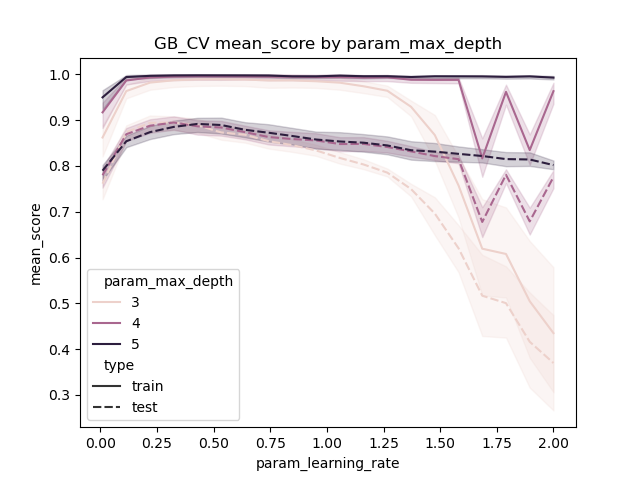
\includegraphics[width=.95\textwidth]{../results5/gb_cv/param_max_depth_mean_score_param_learning_rate.png}
    \caption{GB Performance by Learning Rate}
    \end{subfigure}%
  \begin{subfigure}{.5\textwidth}
    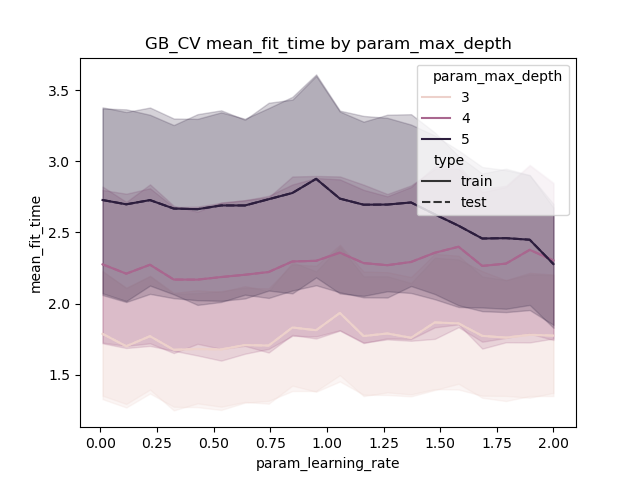
\includegraphics[width=.95\textwidth]{../results5/gb_cv/param_max_depth_mean_fit_time_param_learning_rate.png}
    \caption{GB Average Fit Time by Learning Rate}
  \end{subfigure}
  \begin{subfigure}{.5\textwidth}
    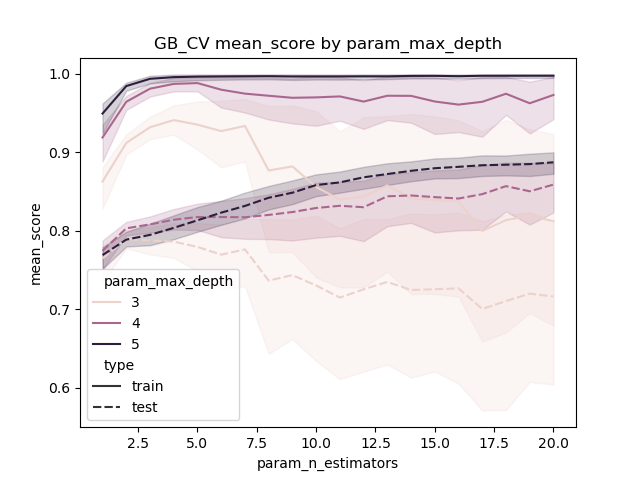
\includegraphics[width=.95\textwidth]{../results5/gb_cv/param_max_depth_mean_score_param_n_estimators.png}
    \caption{GB Performance by Estimators}
    \end{subfigure}%
  \begin{subfigure}{.5\textwidth}
    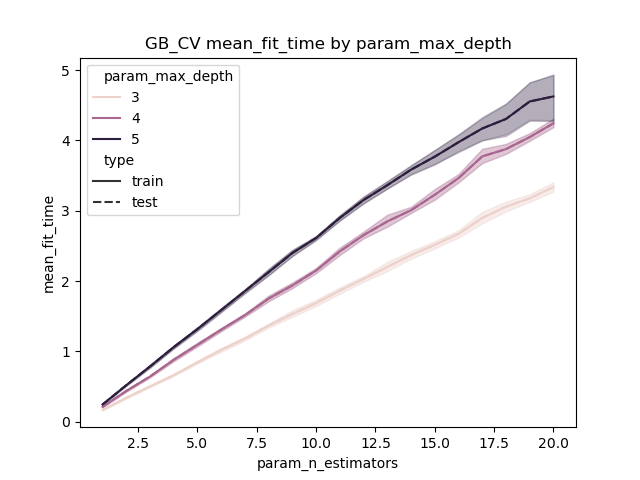
\includegraphics[width=.95\textwidth]{../results5/gb_cv/param_max_depth_mean_fit_time_param_n_estimators.png}
    \caption{GB Average Fit Time by Estimators}
  \end{subfigure}
  \caption{GB Performance}
  \label{figure5}
\end{figure}

\subsection{c)}

\begin{figure}
  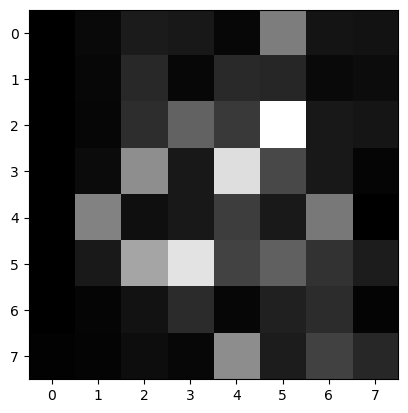
\includegraphics[width = .75\textwidth]{../results5/Features_Digits.png}
  \caption{Feature Importances Image}
  \label{figure6}
\end{figure}

Looking at the relevant features for the GB classifier in Figure \ref{figure6}, we can see that we have our work cut out 
for us. This mapping of relevance likely doesn't immediately evoke many connections to someone looking at it. However,
if we look closely we can see a method to the madness. 

When drawing a number, humans will likely make "errors" in the direction that we were already going to move our pencil, 
and we are usually more likely to overflow in the direction of our writing. Most people naturally write from top left to 
bottom right when making connected movements. For example, think about how you would draw a 2, 3, or 5. Most people 
start in the top left corner of the number, and move to the bottom right. You might think that the 5 is an exception because 
many people draw the lower part of the 5 followed by the horizontal line. But this is what I mean by "connected movements", 
since draing the bottom part of the 5 goes from top to bottom, and the hat goes from left to right. 

Following these ideas of how people draw images and make errors, we can see that the image begins to make sense. The 
bottom right quadrant of the image appears to be more important overall, which is where we'd expect to see a lot of 
unique errors relating to how the number is drawn. Thinking critically, we can estimate that the numbers 2, 3, 5, 6, and 9 are 
far more likely to have items overflowing to the bottom right than the other numbers. 

Looking at the pixel at (0,5), we can consider the fact that this would only realistically be activated by a 1, 5, 6 
or 7. In addition, if we look at the highly activated pixels in the center of the image, we can see that these would be 
activated differently by 0, 4, 5, and 8 than the other numbers. With all of this in mind, we now have a vague idea of 
different regions of activation that could be connected to what number is being written.

\subsection{d)}
To begin identifying missed samples, I used a Confusion Matrix to get an idea of how many samples we missed and how 
common the errors were. We can see this in Figure \ref{figure7}. We can see that we performed quite well, with no 
combination having more than 2 samples missclassified in the same way. Moving on from this matrix since it wasn't 
directly requested in the exam, and I am tired, we arrive at the plot of one missed sample from each class, and the table 
that contains the neighbor information.

\begin{figure}
  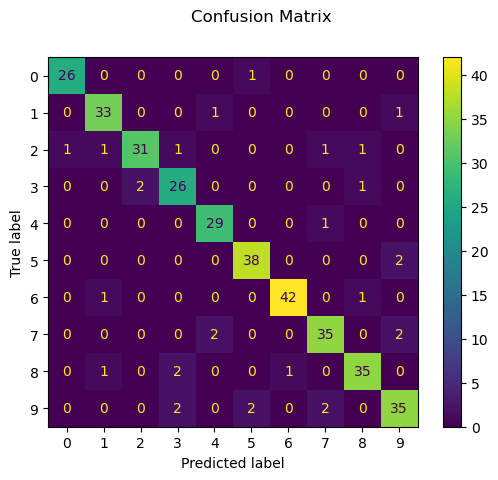
\includegraphics[width = \textwidth]{../results5/Digits_Confusion.png}
  \caption{Confusion Matrix}
  \label{figure7}
\end{figure}

\begin{figure}
  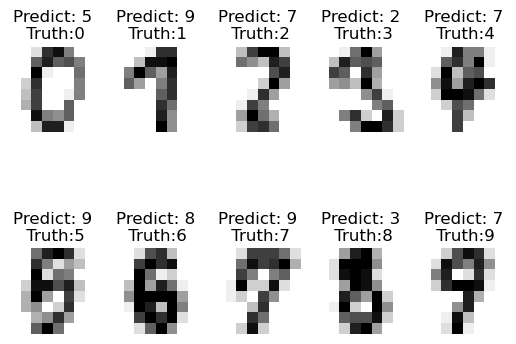
\includegraphics[width = \textwidth]{../results5/Digits_Missed.png}
  \caption{Missed Examples}
  \label{figure8}
\end{figure}

Looking at Figure \ref{figure8}, we can see some examples of missed samples sorted by their true value. Starting with 0, 
we can see that the left side and the bottom of the 0 are more activated than the upper right side of the 0, which is likely 
why it was predicted as a 5. Looking at the top 3 neighbors, we see that actually all 3 of them are the correct class. 
I think this is evidence of a weakness in the model.

For number 1, we can see that this 1 had a very long upper hat that was primarily spread out on a diagonal. This can 
lead the result to look like a 9 with a small loop. Overall, I'd say this should have been more likely predicted as a
7 in my opinion, but I can see how a 9 would arise. Much like the 0, this also had the top 3 neighbors labelled correctly.
Another evidence of a weakness in the model.


\begin{table}
  \resizebox*{\textwidth}{!}{\begin{tabular}{rrrrrrrrrr}
\toprule
 truth &  pred &  idx &  Neigbor\#1\_True Class &  Neigbor\#1\_Distance &  Neigbor\#2\_True Class &  Neigbor\#2\_Distance &  Neigbor\#3\_True Class &  Neigbor\#3\_Distance &  Neighbor\_average\_Distance \\
\midrule
     0 &     5 &  307 &                     0 &              0.5900 &                     0 &              0.6000 &                     0 &              0.6000 &                     0.5977 \\
     1 &     9 &  213 &                     1 &              0.5900 &                     1 &              0.6500 &                     1 &              0.6600 &                     0.6301 \\
     2 &     7 &   66 &                     3 &              0.7300 &                     7 &              0.7900 &                     7 &              0.8000 &                     0.7728 \\
     3 &     2 &  185 &                     3 &              0.4300 &                     9 &              0.6900 &                     3 &              0.7000 &                     0.6083 \\
     4 &     7 &  315 &                     4 &              0.6700 &                     7 &              0.7800 &                     7 &              0.7900 &                     0.7459 \\
     5 &     9 &   84 &                     5 &              0.8400 &                     5 &              0.8600 &                     5 &              0.8600 &                     0.8547 \\
     6 &     8 &   47 &                     6 &              0.6300 &                     6 &              0.7100 &                     6 &              0.7500 &                     0.6971 \\
     7 &     9 &   21 &                     7 &              0.3500 &                     7 &              0.4300 &                     7 &              0.5100 &                     0.4286 \\
     8 &     3 &  122 &                     3 &              0.8500 &                     6 &              0.8600 &                     3 &              0.9200 &                     0.8767 \\
     9 &     7 &  115 &                     9 &              0.5300 &                     9 &              0.5400 &                     9 &              0.6200 &                     0.5629 \\
\bottomrule
\end{tabular}
}
  \caption{Neighbors of missed samples}
  \label{table3}
\end{table}

For number 2, This was missclassified as a 7. I can totally see why. I could be convinced that was a 7 with a mistake myself.
Regardless, it definitely doesn't look like a 2 very clearly to me. The neighbors seemed to agree, with the top neighbor 
appearing as 3, and the next 2 appearing as a 7. I'd say that this is a good example of a bad sample that's understandable to miss.

For number 3, I think that this is a terrible 3. This does not look like much that's understandable, and personally I count 
it as a win since it shows errors exactly how I predicted people would make mistakes in section 5a. Looking at the neighbors,
we can see it did have a pretty close neighbor that was correct, but that it also shared a 9. Even though the neighbors seem 
to be doing alright, I personally would say that this sample is uncharacteristic of most 3's and is an outlier.

For number 4, this looks awful. I wouldn't even consider this to be a number. Both the predicted value and the nearest 
neighbors agree that this looks like a 7, but I'd say that this is mostly because it vaguely has a higher concentation 
at the top right going down to the bottom middle, which a 7 is the most likely to have.

For number 5, this sample looks quite noisy. We can see the 5 in there, but almost the whole grid is activated in some 
noticeable way. Admittedly, all of the top neighbors are correct, but they have the second largest average distance 
of any of the numbers, which supports that this is an outlier due to noise.

For number 6, I think that the model mistook it for an 8 because of the raw amount of activation. Given my normalization, 
these strong amount of activation would have been squashed which I can understand how it would lead to a missclassification 
of this sample. However, all of the nearest neighbors are correct, so I'd say that this one is likely a mistake due to my choice
of normalization.

For number 7, I think this one is an examplee of the weakness of this model. The number 7 and number 9 have shown up the 
most consistently of any of the numbers so far, and it appears that the model struggled the most with number 7 and 9. 
As such, it makes sense that the model would struggle with confusing 7's and 9's (which we will see again at 9).
This number most closely clusters with it's neighbors, and visually can be understood as a 7 with only moderate effort.
I think this is an example of a weakness in the model.

For number 8, I can understand the mistake because there's no middle loop for the 8. That's a very important feature of 
the number that this sample doesn't have. You can see the problem in the neighbors where none of them are correct, 
and they have the largest average distance of any number.

Finally, for number 9, there's honestly no excuse for the model to get this wrong. This is clearly a clean 9, and all of 
the neighbors are correct. This is a strong evidence for the consistent problem of our model confusing 7's and 9's. I 
hate to end on such a strong negative point, but this is a problem that would have to be addressed if we were trying to 
push this model into production somewhere for some reason. Likely, the problem is that this 9 is too far to the right,
where we can see in the feature importances image our model is largely ignoring. 

\end{document}